\subsection{Das OSI-Refernezmodell}
Das OSI-Schichtenmodell ist ein Modell zur Veranschaulichung komplexer Kommunikationssysteme.
Komplex bedeutet hierbei, dass sich das Modell mit der Kommunikation zwischen verschiedenen Computersystemen in einem Netzwerk beschäftigt.
Das Modell besteht aus sieben Schichten (auch Ebenen oder Layer genannt), die verschiedene Instanzen enthalten, welche wiederum unterschiedliche Dienste (Services) bereitstellen.

\begin{figure}[htbp]
    \centering
    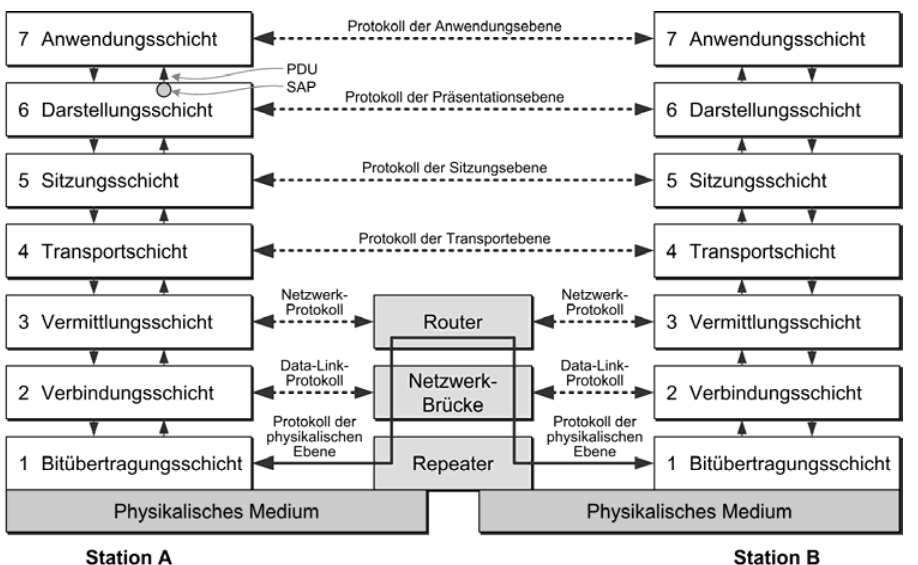
\includegraphics[width=\Bildbreite]{Grafiken/OSI.png}
    \caption{OSI-Modell}
    \label{fig: OSI}
\end{figure} 

Kommunikation zwischen den Schichten
Die Kommunikation der Schichten untereinander erfolgt über sogenannte Dienstzugangspunkte (Service Access Points, SAPs). Dabei ist zu beachten, dass das Ziel darin besteht, dass eine höhere Schicht Daten von den Diensten der darunterliegenden Schichten anfordern oder empfangen kann. Die untere Schicht dient somit als Dienstleister für die obere Schicht.

Um Daten anzufordern oder zu empfangen, werden sogenannte Dienstelemente verwendet. Es ist außerdem wichtig zu wissen, dass eine Schicht mehrere Instanzen und Dienste besitzen kann.

Kommunikation innerhalb einer Schicht
Instanzen innerhalb einer Schicht können über Protokolle miteinander kommunizieren. Dies ermöglicht:

die Bereitstellung eines Dienstes durch die Zusammenarbeit zweier Instanzen, oder
eine effizientere Fehlersuche, da Problemquellen besser isoliert werden können.
Zur Unterscheidung der verschiedenen Dienste werden Service Access Point Identifier (SAPI) verwendet, die bei Anfragen oder beim Empfangen von Daten mit angegeben werden.

Kommunikation zwischen Geräten
Die Kommunikation zwischen zwei Geräten erfolgt über sogenannte PDUs (Protocol Data Units).
Möchte Gerät A Daten an Gerät B senden, erstellt Gerät A in der obersten Schicht eine PDU. Diese PDU wird mit Kontrollinformationen ergänzt und an die nächstuntere Schicht weitergeleitet. Dieser Vorgang wiederholt sich, bis die unterste Schicht erreicht ist.

Die PDU wird dann über das Übertragungsmedium (z. B. Kabel oder Funk) an Gerät B gesendet. Dort wird die PDU von der untersten Schicht entgegengenommen, und jede Schicht überprüft nacheinander die für sie relevanten Kontrollinformationen. Am Ende erhält die oberste Schicht von Gerät B die ursprünglichen Daten.


\subsection{Physikalische Schicht}
CAN-Bus deckt in diesem Modell nur die ersten beiden Schichten ab. CAN deckt die erste Schicht, die physikalische Schicht, ab da ganz klar geregelt ist wie die Übertragung der einzelnen Bits stattfindet. 

\subsection{Sicherungsschicht}
Die zweite Schicht, die Sicherungsschicht wird ebenfalls abgedeckt. Damit diese Schicht abgedeckt wird müssen die Daten in einer klaren Form verpackt werden so das Übertragungsfehler von den Teilnehmenr erkannt werden können. Dies wird im CAN-Bus durch den klaren Aufbau des CAN-Telegrams und das Fehlermanagement gewährleistet.